\subsection*{Box-and-Pointer Diagrams}

So far, we've been working with fairly simple lists whose contents we can
visualize in our heads. With the introduction of list mutation, programs
containing multiple list objects, especially nested lists, become very difficult
to keep track of.

To help us better visualize such programs, we can draw \define{box-and-pointer
diagrams} for lists. In a box-and-pointer diagram, each element in the list
goes into a box. The boxes are chained together to create a sequence.
Primitive values, like numbers, are written directly into the box.
Non-primitive values, such as other lists, are drawn outside of the box and are
pointed to with an arrow. You can also label each box with its index to make it
easier to read.

Below is a diagram for the following code:

\begin{lstlisting}
lst1 = [1, 2, 3]
lst2 = [5, lst1, 6]
lst2[2] = [7, 8, 9]
\end{lstlisting}

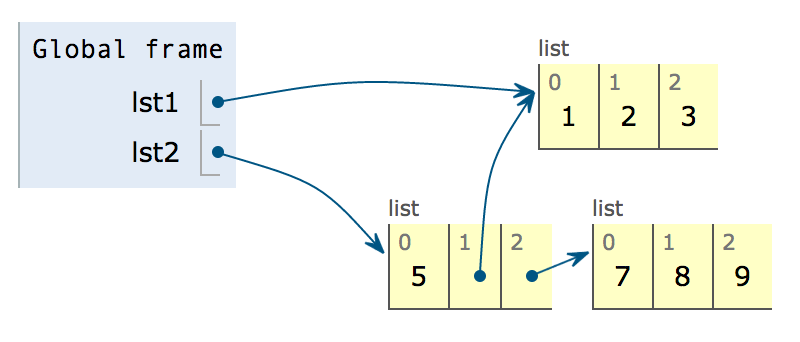
\includegraphics[width=280pt]{box-and-pointer.png} \\
